\documentclass[]{beamer}
\usefonttheme{professionalfonts}
% Class options include: notes, notesonly, handout, trans,
%                        hidesubsections, shadesubsections,
%                        inrow, blue, red, grey, brown

% Theme for beamer presentation.
\usepackage{beamerthemetree}
% Other themes include: beamerthemebars, beamerthemelined, 
%                       beamerthemetree, beamerthemetreebars  

\title{Orbital Optimization in Valence Bond Theory}
\author{Jeroen Engelberts}
%\institute{SURFsara}
\date{9 September 2013}
\titlegraphic{\vspace{20px}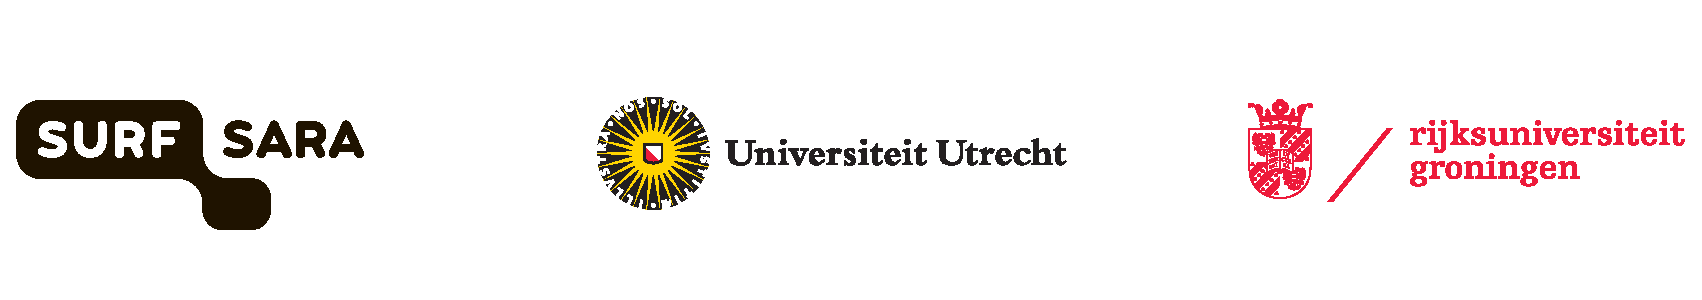
\includegraphics[scale=0.38]{figures/logos.eps}}

\begin{document}

\begin{frame}
  \titlepage
\end{frame}

\begin{frame}
  \frametitle{Goal}
  Analyze the orbital optimization process in the Valence Bond Self Consistent Field (VBSCF) method and look for possibilities to improve the performance, \textit{i.e.} decrease the computation time.
\end{frame}

\begin{frame}
  \tableofcontents
\end{frame}

\section{Valence Bond Theory}

\subsection{Valence Bond Wave Functions}

\begin{frame}
  \frametitle{Single Structure Wave Function}
  \begin{center}
    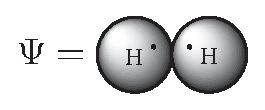
\includegraphics{figures/heitler.eps}  
  \end{center}
  \begin{equation*}
    \Psi = N \{ |1s_{A}\overline{1s_{B}}| - |\overline{1s_{A}}1s_{B}| \}
  \end{equation*}
  \begin{itemize}
    \item {Introduced by Heitler and London in 1927}
    \item {Describes covalent bond in H$_2$}
    \item {Based on spin-pairing}
    \item {Multi-determinant}
  \end{itemize}
\end{frame}

\begin{frame}
  \frametitle{Multiple Structure Wave Function}
  \begin{center}
    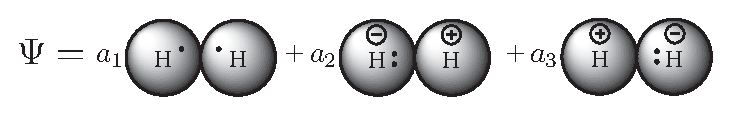
\includegraphics[scale=0.95]{figures/heitlerplus.eps}
  \end{center}
  \begin{equation*}
    \Psi= N \{ a_1(|1s_{A}\overline{1s_{B}}| - |\overline{1s_{A}}1s_{B}|) + a_2 |1s_{A}\overline{1s_{A}}| + a_3 |1s_{B}\overline{1s_{B}}| \}
  \end{equation*}
  \begin{itemize}
    \item {Versatility is added by expanding with more structures}
    \item {$a_2 = a_3$, for homonuclear diatomic molecules}
    \item {Heteronuclear - ionic contribution will differ ($a_2 \neq a_3$)}
  \end{itemize}
\end{frame}

\begin{frame}
  \frametitle{Coulson-Fischer Type Wave Function}
  \begin{center}  
    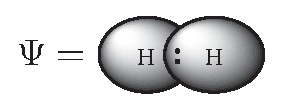
\includegraphics{figures/coulson.eps}
  \end{center}
  \begin{equation*}
    \Psi = N \{ | \phi_1 \overline{\phi_2} | - | \overline{\phi_1} \phi_2 | \}
  \end{equation*}
  \begin{center}
    where $\phi_1 = 1s_A + \lambda_1 1s_B$ and $\phi_2 = 1s_B + \lambda_2 1s_A$
  \end{center}  
  \begin{itemize}
    \item {Introduced by Coulson and Fischer in 1949}
    \item {CF orbitals are spread over atoms (unless $\lambda$'s are zero)}
    \item {For polar diatomic molecules, the $\lambda$'s will differ}
  \end{itemize}
\end{frame}

\begin{frame}
  \frametitle{Modern Valence Bond Wave Functions}
  \begin{tabular}{ll}
    $\Psi = \sum_{i} C_i \Phi_i$ & WF: linear combination of structures \\
    $\Phi = \sum_{i} \alpha_i \Delta_i$ & Structure: linear combination of determinants \\
    $\Delta = |\phi_i\phi_j\phi_k\phi_l \cdots \phi_n|$ & Determinant: subset of molecular orbitals \\
    $\phi = \sum_{n} c_n \chi_n$ & MO: linear combination of atomic orbitals
  \end{tabular}
  \vspace{15px}
  \begin{center}
    The wave function can be modified/enhanced in two spots
  \end{center}
\end{frame}

\begin{frame}
  \frametitle{Modern Valence Bond Wave Functions}
  \begin{tabular}{ll}
    \textcolor{red}{$\Psi = \sum_{i} C_i \Phi_i$} & \textcolor{red}{WF: linear combination of structures} \\
    \textcolor{gray}{$\Phi = \sum_{i} \alpha_i \Delta_i$} & \textcolor{gray}{Structure: linear combination of determinants} \\
    \textcolor{gray}{$\Delta = |\phi_i\phi_j\phi_k\phi_l \cdots \phi_n|$} & \textcolor{gray}{Determinant: subset of molecular orbitals} \\
    \textcolor{gray}{$\phi = \sum_{n} c_n \chi_n$} & \textcolor{gray}{MO: linear combination of atomic orbitals}
  \end{tabular}
  \vspace{15px}
  \begin{center}
    The coefficients for the structures $C_i$ can be optimized
  \end{center}
\end{frame}

\begin{frame}
  \frametitle{Modern Valence Bond Wave Functions}
  \begin{tabular}{ll}
    \textcolor{gray}{$\Psi = \sum_{i} C_i \Phi_i$} & \textcolor{gray}{WF: linear combination of structures} \\
    \textcolor{gray}{$\Phi = \sum_{i} \alpha_i \Delta_i$} & \textcolor{gray}{Structure:  linear combination of determinants} \\
    \textcolor{gray}{$\Delta = |\phi_i\phi_j\phi_k\phi_l \cdots \phi_n|$} & \textcolor{gray}{Determinant: subset of molecular orbitals} \\
    \textcolor{red}{$\phi = \sum_{n} c_n \chi_n$} & \textcolor{red}{MO: linear combination of atomic orbitals}
  \end{tabular}
  \vspace{15px}
  \begin{center}
    The orbitals can be optimized by modifying $c_n$ in a clever way
  \end{center}
\end{frame}

\begin{frame}
  \frametitle{Construction Of A VB Wave Function}
  \begin{enumerate}
    \item {Create an optimal geometry (mostly with a cheaper method)}
    \item {Obtain initial orbitals with RHF (core orbitals)}
    \item {Define active orbitals by hand}
    \item {Split orbitals in an appropriate number of fragments}
    \item {Choose a meaningful number of structures}
    \item {Optimize the wave function ($C_i$ and $c_n$)}
  \end{enumerate}
  \begin{center}
    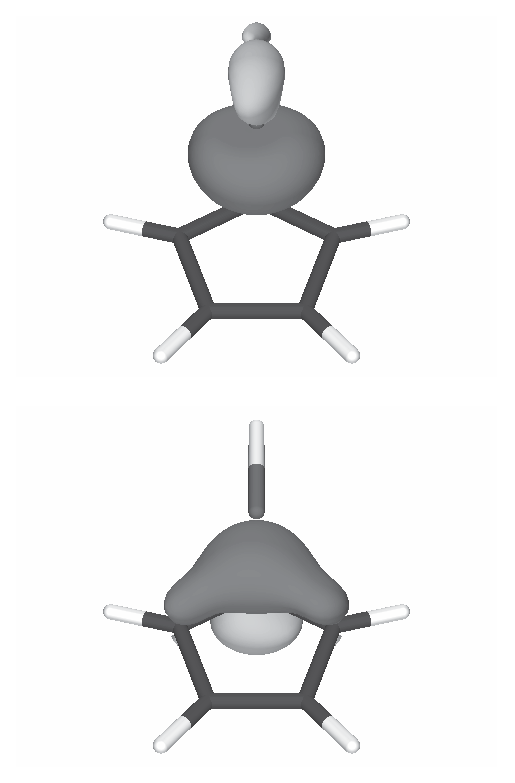
\includegraphics[scale=0.4]{figures/sigma_sih.eps}
  \end{center}
\end{frame}

\subsection{Adapting Orbitals}

\begin{frame}
  \frametitle{Adapting Orbitals}
  \setbeamercolor{normal text}{fg=gray,bg=}
  \setbeamercolor{alerted text}{fg=black,bg=}
  \usebeamercolor{normal text}
  \begin{itemize}  
    \item \alert<+> {Imagine a (molecular) orbital $\phi_i$}
    \item \alert<+> {Let's add a small fraction ($\delta b_{ia}$) of orbital $\phi_a$}
    \item \alert<+> {$\phi_i' = \phi_i + \delta b_{ia} \phi_a$}
    \item \alert<+> {A determinant containing $\phi_i$, like $|\phi_i\overline{\phi_i}\phi_j\phi_k|$, becomes}
    \item \alert<+> {$|\phi_i'\overline{\phi_i'}\phi_j\phi_k | = |(\phi_i + \delta b_{ia} \phi_a)\overline{(\phi_i + \delta b_{ia} \phi_a)}\phi_j\phi_k|$}
    \item \alert<+> {$|\phi_i'\overline{\phi_i'}\phi_j\phi_k | = |\phi_i\overline{\phi_i}\phi_j\phi_k| + \delta b_{ia}|\phi_a\overline{\phi_i}\phi_j\phi_k| + \delta b_{ia} |\phi_i\overline{\phi_a}\phi_j\phi_k| + \delta b^2_{ia} |\phi_a\overline{\phi_a}\phi_j\phi_k|$}
  \end{itemize}
\end{frame}

\begin{frame}
  \frametitle{Adapting Orbitals}
  \setbeamercolor{normal text}{fg=gray,bg=}
  \setbeamercolor{alerted text}{fg=black,bg=}
  \usebeamercolor{normal text}
  \begin{itemize}  
    \item \alert<+> {Since $\delta b_{ia}$ is small, $\delta b^2_{ia}$ is negligible, and so}
    \item \alert<+> {$|\phi_i'\overline{\phi_i'}\phi_j\phi_k | = |\phi_i\overline{\phi_i}\phi_j\phi_k| + \delta b_{ia}|\phi_a\overline{\phi_i}\phi_j\phi_k| + \delta b_{ia} |\phi_i\overline{\phi_a}\phi_j\phi_k|$}
    \item \alert<+> {If $\Psi_{(0)} = |\phi_i\overline{\phi_i}\phi_j\phi_k|$, then}
    \item \alert<+> {$\Psi_{(0)}' = \Psi_{(0)} + \delta b_{ia} \Psi_{ia}$, where}
    \item \alert<+> {$\Psi_{ia}=|\phi_a\overline{\phi_i}\phi_j\phi_k| + |\phi_i\overline{\phi_a}\phi_j\phi_k|$}
    \item \alert<+> {In general: $\Psi_{(0)}'=\Psi_{(0)}+\sum_i\sum_{a} \delta_{ia} \Psi_{ia}$, where}
    \item \alert<+> {$i$ runs over all occupied orbitals, $a$ over all unoccupied orbitals}
  \end{itemize}
\end{frame}

\section{Orbital Optimization}

\subsection{Super CI}

\begin{frame}
  \frametitle{Super CI}
  \setbeamercolor{normal text}{fg=gray,bg=}
  \setbeamercolor{alerted text}{fg=black,bg=}
  \usebeamercolor{normal text}
  Adaption OK, but how to improve the wave function?
  \begin{enumerate}  
    \item \alert<+> {Calculate $C_i$ in $\Psi_0 = \sum_{i} C_i \Phi_i$, with:}
    \item \alert<+> {$[\mathbf{H}-E\mathbf{S}] \cdot \mathbf{C} = 0$}
    \item \alert<+> {Expand the wave function with Brillouin states, $\Psi_{ia}$}
    \item \alert<+> {$\Psi_{superci} = \Psi_0 + \sum_{ia,a \neq i} b_{ia}\Psi_{ia}$}
    \item \alert<+> {Solve the eigenvalue problem to obtain values for $\mathbf{b}$}
    \item \alert<+> {$[\mathbf{H}-E_b\mathbf{S}] \cdot \mathbf{b} = 0$}
    \item \alert<+> {Update orbitals with elements from $\mathbf{b}$:}
    \item \alert<+> {$\phi_i \leftarrow \phi_i + \sum_{a,a \neq i} b_{ia}\phi_a$}
    \item \alert<+> {Start from step 1, unless converged}
  \end{enumerate}
\end{frame}

\begin{frame}
  \frametitle{Super CI}
  Updating the orbitals of the earlier example $\Psi_0$
  \begin{equation*}
    \begin{split}
      \Psi_{0} \leftarrow & \Psi_{0} + b_{ia} \Psi_{ia} = \\
      &|\phi_i\overline{\phi_i}\phi_j\phi_k| + b_{ia}(|\phi_a\overline{\phi_i}\phi_j\phi_k| + |\phi_i\overline{\phi_a}\phi_j\phi_k|) = \\
      &|(\phi_i + b_{ia}\phi_a)\overline{(\phi_i + b_{ia}\phi_a)}\phi_j\phi_k| = \\
      &|\phi_i'\overline{\phi_i'}\phi_j\phi_k |
    \end{split}
  \end{equation*}
\end{frame}

\subsection{Brillouin Theorem}

\begin{frame}
  \frametitle{Brillouin Theorem}
  When are the orbitals optimal?
  \begin{equation*}
    \begin{split}
      \frac{\partial E}{\partial b_{ia}} & =\frac{\partial \frac{\left < \Psi_0 | \mathbf{H} | \Psi_0 \right >}{\left < \Psi_0 | \Psi_0 \right >}}{\partial b_{ia}}\\
      & = \frac{2 \cdot \left < \Psi_0 | \mathbf{H} | \Psi_{ia} \right > \left< \Psi_0 | \Psi_0 \right > - 2 \cdot \left < \Psi_0 | \mathbf{H} | \Psi_0  \right > \left< \Psi_0 | \Psi_{ia}\right>}{\left < \Psi_0 | \Psi_0 \right > ^2 }\\
      & = \frac{ 2 \cdot \left < \Psi_0 | \mathbf{H} | \Psi_{ia} \right > - 2 \cdot E_0 \left< \Psi_0 | \Psi_{ia} \right >}{\left < \Psi_0 | \Psi_0 \right >}\\
      & = \frac{ 2 \cdot \left < \Psi_0 | \mathbf{H} -E_0 | \Psi_{ia} \right >}{\left < \Psi_0 | \Psi_0 \right >}\\
      & = 0
    \end{split}
  \end{equation*}
\end{frame}

\subsection{Implementation}

\begin{frame}[fragile]
  \begin{verbatim}
   t                      t       l                               
   t                      t       l                               
  tttt    u  u   rrrrr   tttt     l         eee   
   t      u  u    r   r   t       l        eeeee  
   t   t  u  u    r       t   t   l   l    e      
    ttt    uu     r        ttt     lll      eee    


         ----           ----   )))))             
  ----         ----   _ _ _   { o o }     
          ----      _(_)_(_)_  ( ^ )              
-                 _(_)_(_)_(_)_/ /                        
                _(_)_(_)_(_)_(_)/                       
               (_)_(_)_(_)_(_)_(_)                     
  ----           //  //   //  //           
  \end{verbatim}
\end{frame}

\begin{frame}
  \frametitle{Construction of $\mathbf{H}$ and $\mathbf{S}$}
  \setbeamercolor{normal text}{fg=gray,bg=}
  \setbeamercolor{alerted text}{fg=black,bg=}
  \usebeamercolor{normal text}
  \begin{itemize}  
    \item \alert<+> {To calculate $[\mathbf{H}-E_b\mathbf{S}] \cdot \mathbf{b} = 0$, we need $\mathbf{H}$ and $\mathbf{S}$}
    \item \alert<+> {\begin{equation*}\left[\begin{array}{ccc}\left< \Psi_{0} | \mathbf{H} - E_0 | \Psi_{0} \right> & \left< \Psi_{ia} | \mathbf{H} - E_0 | \Psi_{0} \right> & \left< \Psi_{ib} | \mathbf{H} - E_0 | \Psi_{0} \right> \\
                    \left< \Psi_{0} | \mathbf{H} - E_0 | \Psi_{ia} \right> & \left< \Psi_{ia} | \mathbf{H} - E_0 | \Psi_{ia} \right> & \left< \Psi_{ib} | \mathbf{H} - E_0 | \Psi_{ia} \right> \\
                    \left< \Psi_{0} | \mathbf{H} - E_0 | \Psi_{ib} \right> & \left< \Psi_{ia} | \mathbf{H} - E_0 | \Psi_{ib} \right> & \left< \Psi_{ib} | \mathbf{H} - E_0 | \Psi_{ib} \right> \\
                    \end{array}\right]
                    \end{equation*}}
        \item \alert<+> {\begin{equation*}\left[\begin{array}{ccc}\left< \Psi_{0} | \Psi_{0} \right> & \left< \Psi_{ia} | \Psi_{0} \right> & \left< \Psi_{ib} | \Psi_{0} \right> \\
                    \left< \Psi_{0} | \Psi_{ia} \right> & \left< \Psi_{ia} | \Psi_{ia} \right> & \left< \Psi_{ib} | \Psi_{ia} \right> \\
                    \left< \Psi_{0} | \Psi_{ib} \right> & \left< \Psi_{ia} | \Psi_{ib} \right> & \left< \Psi_{ib} | \Psi_{ib} \right> \\
                    \end{array}\right]
                    \end{equation*}}
    \item \alert<+> {$n$ excitations $\rightarrow$ $\frac{n(n+1)}{2}$ elements for $\mathbf{H}$ and $\mathbf{S}$}
  \end{itemize}
\end{frame}

\begin{frame}
  \frametitle{Construction of Matrix Elements}
  \begin{equation*}
    \begin{split}
      \left < \Psi_0 | \mathbf{H} - E_0 | \Psi_{ia} \right>= & + N^2 \sum_{\rho\tau} h_{\rho\tau} \sum_{xy} S_{xy}^{(\rho,\tau)}\gamma_x\gamma_y \\
      & + N^2 \sum_{\rho<\sigma,\tau<\nu} [\left <\rho\sigma|\tau\nu \right > - \left < \rho\sigma | \nu\tau \right> ] \sum_{xy} S_{xy}^{(\rho,\sigma,\tau,\nu)}\gamma_x\gamma_y \\
      &  - E_0 N^2 \sum_{xy} S_{xy}^{(0)}\gamma_x\gamma_y \\
    \end{split}
  \end{equation*}
  Where
  \begin{itemize}
    \item {$h_{\rho\tau} = \left< \phi_\rho(1) | \mathbf{h} | \phi_\tau(1) \right>$}
    \item {$\left<\rho\sigma | \tau\nu \right> = \left<\phi_\rho(1)\phi_\sigma(2) | \frac{1}{r_{12}} | \phi_\tau(1)\phi_\nu(2) \right>$}
  \end{itemize} 
\end{frame}

\begin{frame}
  \frametitle{An Example Of A Cofactor (zeroth order)}
  \begin{itemize}
    \item $\Psi_0 = |ijkl...n|$
    \item $\Psi_{ia} = |ajkl...n|$
    \item $s_{ia} = \left< \phi_i | \phi_a \right>$
  \end{itemize}
  \begin{equation*}
S_{0(i \rightarrow a)}^{(0)}=
\begin{array}{lllllll}
 &  i & j & k & l & \cdots & n \\
 a &  \multicolumn{1}{|l}{s_{ia}} & s_{ja}  & s_{ka} & s_{la} & & \multicolumn{1}{l|}{ s_{na} } \\
 j & \multicolumn{1}{|l}{s_{ij}} & 1 & s_{kj} & s_{lj} & & \multicolumn{1}{l|}{s_{nj}} \\
 k & \multicolumn{1}{|l}{s_{ik}} & s_{jk} & 1 & s_{lk} & & \multicolumn{1}{l|}{s_{nk}} \\
 l & \multicolumn{1}{|l}{s_{il}} & s_{jl} & s_{kl} & 1 & & \multicolumn{1}{l|}{s_{nl}} \\
 \vdots & \multicolumn{1}{|l}{ } &   &   & & \ddots & \multicolumn{1}{l|}{\vdots} \\
 n & \multicolumn{1}{|l}{ s_{in}} & s_{jn} & s_{kn} & s_{ln} & \cdots & \multicolumn{1}{l|}{1}
\end{array}
  \end{equation*}
\end{frame}

\begin{frame}
  \frametitle{An Example Of A Cofactor (first order)}
  \begin{itemize}
    \item $\Psi_0 = |ijkl...n|$
    \item $\Psi_{ia} = |ajkl...n|$
    \item $s_{kj} = \left< \phi_k | \phi_j \right>$
  \end{itemize}
  \begin{equation*}
S_{0(i \rightarrow a)}^{(i,a)}=
\begin{array}{llllll}
 & j & k & l & \cdots & n \\
 j & \multicolumn{1}{|l}{1} & s_{kj} & s_{lj} & & \multicolumn{1}{l|}{s_{nj}} \\
 k & \multicolumn{1}{|l}{s_{jk}} & 1 & s_{lk} & & \multicolumn{1}{l|}{s_{nk}} \\
 l & \multicolumn{1}{|l}{s_{jl}} & s_{kl} & 1 & & \multicolumn{1}{l|}{s_{nl}} \\
 \vdots & \multicolumn{1}{|l}{ } &   & & \ddots & \multicolumn{1}{l|}{\vdots} \\
 n & \multicolumn{1}{|l}{ s_{jn}} & s_{kn} & s_{ln} & \cdots & \multicolumn{1}{l|}{1}
\end{array}
  \end{equation*}
\end{frame}

\begin{frame}
  \frametitle{An Example Of A Cofactor (second order)}
  \begin{itemize}
    \item $\Psi_0 = |ijkl...n|$
    \item $\Psi_{ia} = |ajkl...n|$
    \item $s_{kj} = \left< \phi_k | \phi_j \right>$
  \end{itemize}
  \begin{equation*}
S_{0(i \rightarrow a)}^{(i,k,a,l)}=
\begin{array}{lllll}
 & j & k & \cdots & n \\
 j & \multicolumn{1}{|l}{1} & s_{kj} & & \multicolumn{1}{l|}{s_{nj}} \\
 l & \multicolumn{1}{|l}{s_{jl}} & s_{kl} & & \multicolumn{1}{l|}{s_{nl}} \\
 \vdots & \multicolumn{1}{|l}{ } & & \ddots & \multicolumn{1}{l|}{\vdots} \\
 n & \multicolumn{1}{|l}{ s_{jn}} & s_{kn} & \cdots & \multicolumn{1}{l|}{1}
\end{array}
  \end{equation*}
\end{frame}

\section{Approximated Newton-Raphson}

\begin{frame}
  \frametitle{Approximated Newton-Raphson}
  \setbeamercolor{normal text}{fg=gray,bg=}
  \setbeamercolor{alerted text}{fg=black,bg=}
  \usebeamercolor{normal text}
  Can we reach the Brillouin condition with less matrix elements?
  \begin{itemize}
    \item \alert<+> {In aNR, the orbital update coefficients ($\mathbf{b}$) are approximated:}
    \item \alert<+> {\begin{equation*}b_{ia} = -\frac{\left< \Psi_0 | \mathbf{H} - E_0 | \Psi_{ia} \right>}{\left< \Psi_{ia} | \mathbf{H} - E_0 | \Psi_{ia} \right>}\end{equation*}}
    \item \alert<+> {Elements of the type $\left< \Psi_{ia} | \mathbf{H} - E_0 | \Psi_{ib} \right>$ are not needed}
    \item \alert<+> {$n$ excitations $\rightarrow$ \textit{only} $2n+1$ elements for $\mathbf{H}$ and $\mathbf{S}$}
    \item \alert<+> {But ... does it work as well as Super CI?}
  \end{itemize}
\end{frame}

\subsection{Test Calculations}

\begin{frame}
  \frametitle{Test Calculations}
  \begin{center}
    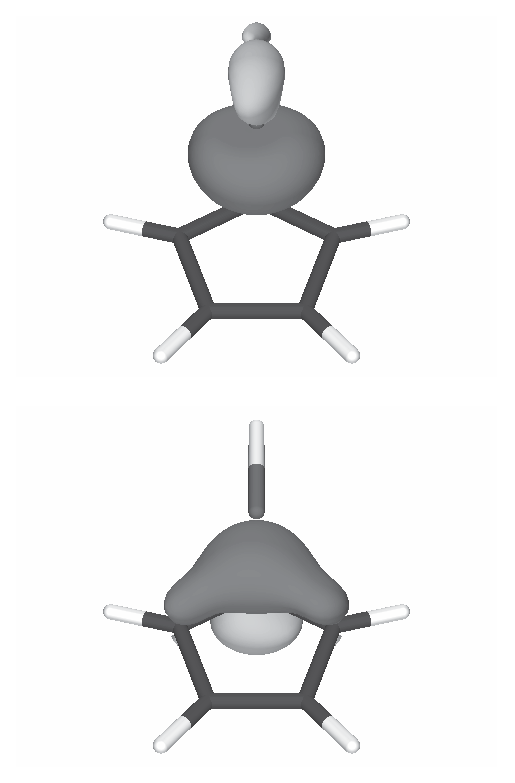
\includegraphics[scale=0.5]{figures/sigma_sih.eps}  
  \end{center}
  \begin{table}
  \begin{center}
    \begin{tabular}{l c c}
      \hline
      Type & no DIIS & DIIS \\
      \hline
      \textit{superci} & 3349 (11) & 2735 (9) \\ 
      \textit{pert} doc-uoc & 1368 (99) & 324 (23)\\ 
      \textit{pert} doc-uoc/voc-uoc & 1172 (98) & 316 (26)\\
    \end{tabular}
  \end{center}
\end{table}
\end{frame}

\section{Fock Matrix Elements}

\begin{frame}
  \frametitle{Fock Matrix Elements}
  Would it be possible to calculate $\mathbf{H}$ and $\mathbf{S}$ elements cheaper?
\end{frame}

\subsection{Test Calculations}

\begin{frame}
  \frametitle{Test Calculations}
  \begin{center}
    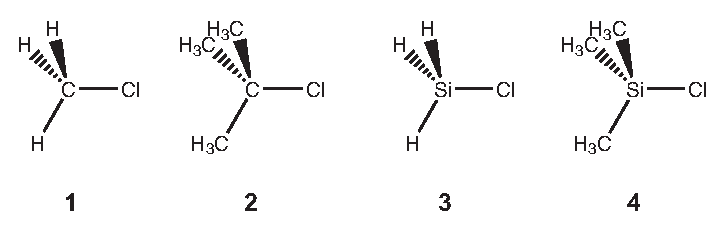
\includegraphics[scale=0.45]{figures/compounds.eps}
  \end{center}
  \begin{table}\small
    \begin{center}
      \begin{tabular}{l c c c c c c}
        \hline
        &\multicolumn{3}{c}{\textbf{Butadiene}}&\multicolumn{3}{c}{\textbf{Benzene}}\\
        &\multicolumn{3}{c}{(-153.59682368 au)}&\multicolumn{3}{c}{(-230.54408700 au)}\\
        \textbf{Method}&\textbf{\# iter}&\textbf{sec/iter}&\textbf{speed-up}&\textbf{\# iter}&\textbf{sec/iter}&\textbf{speed-up}\\
        \hline
        \textit{superci}&8&73.0&1&8&2274.1&1\\
        \textit{pert}&14&4.9&8&13&90.8&15\\
        \textit{fock}&10&4.8&12&10&79.3&23\\
      \end{tabular}
    \end{center}
  \end{table}
\end{frame}

\begin{frame}
  \frametitle{Test Calculations}
  \begin{center}
    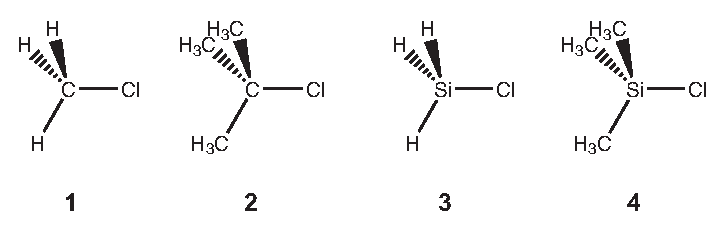
\includegraphics[scale=0.45]{figures/compounds.eps}
  \end{center}
  \begin{table}\small
    \begin{center}
      \begin{tabular}{l c c c c c c}
        \hline
        &\multicolumn{3}{c}{\textbf{Cyclooctatetraene}}&\multicolumn{3}{c}{\textbf{Pentalene}}\\
        &\multicolumn{3}{c}{(-307.35606250 au)}&\multicolumn{3}{c}{(-306.14034868 au)}\\
        \textbf{Method}&\textbf{\# iter}&\textbf{sec/iter}&\textbf{speed-up}&\textbf{\# iter}&\textbf{sec/iter}&\textbf{speed-up}\\
        \hline
        \textit{superci}&8&320106.0&1&8&47692.8&1\\
        \textit{pert}&13&4704.2&42&14&1982.4&14\\
        \textit{fock}&10&3857.0&66&12&1386.8&23\\
      \end{tabular}
    \end{center}
  \end{table}
\end{frame}


\section{Final Remarks}

\begin{frame}
  \frametitle{Remarks}
\end{frame}

\section{Questions And Answers}

\begin{frame}
  \frametitle{Questions And Answers}
  \begin{center}
    \includegraphics[scale=0.85]{figures/questions_answers_5.jpg}  
  \end{center}
\end{frame}

\end{document}
